\chapter{光线追踪}

计算机图形学的一个基本任务就是三维场景的渲染(Redering)。渲染是指,对于一系列排列在三维空间中的物体,产生一张从三维空间特定视角观察这些物体的二维图像。本质上说,渲染是一系列物体为输入以一个像素阵列为输出的过程,无论具体如何实现,渲染总会涉及这样一个问题:每个物体是如何影响每个像素的?渲染有以下两种的主流实现方式
\begin{enumerate}
    \item 物体顺序渲染(Object Order Redering),遍历每个物体,考虑它们会影响哪些像素。
    \item 图像顺序渲染(Image Order Redering),遍历每个像素,考虑它们将如何被物体确定。
\end{enumerate}
若借用计算机语言,渲染即是一个包含遍历物体和遍历像素的双重循环,物体顺序渲染和图像顺序渲染的差别就是哪一循环在外面。两种渲染方式都可以产生相同的图像,但是效率和复杂性是不同的。通常而言,图像顺序渲染更简单也更灵活,不过相较物体顺序渲染需要更长的时间来产生一张图像。本章将研究的光线追踪(Ray Tracking)是一种图像顺序渲染算法。

\section{光线追踪的基本概念}

光线追踪的基本概念可以用\xref{fig:光线追踪的基本概念}来说明,对于每个像素,我们将会产生一条光线,光线的原点和方向与选取的投影方式有关。光线会在三维空间中穿行,光线第一个遇到的物体就代表该像素“看到”的是这个物体,像素就会被渲染为这个物体的颜色。例如在\xref{fig:光线追踪的基本概念}中光线追踪到的是三角面$T_1$。三角面$T_2$未被光线经过,三角面$T_3$在光线上但$T_1$在其前面先遇到光线了。
\begin{Figure}[光线追踪的基本概念]
    \includegraphics[scale=0.8]{build/Chapter04B_03.fig.pdf}
\end{Figure}

因此,简单来说,光线追踪可以分为两个步骤
\begin{enumerate}
    \item 光线产生(Ray Generation),确定每个像素对应的光线的原点和方向。
    \item 光线相交(Ray Intersection),找到最近的与光线相交的物体。
\end{enumerate}
\section{光线产生}
光线产生和投影方式有关,主要有以下两种投影
\begin{itemize}
    \item 平行投影(Parallel Projection),如\cref{fig:平行投影}所示,是指光线从每个像素的中心处发出且所有光线是平行的。平行投影可以分为两种情况,取决于光线方向是否与像平面垂直,分别称为正交投影(Orthographic)和斜交投影(Oblique),其中正交投影比较常见,我们在\cref{fig:平行投影}展示的也是正交投影的情况。平行投影常用于工程图(例如机械和建筑)的绘制,它的最大特征是,三维空间中的平行线经过投影后在二维图像中仍然是平行的。
    \item 透视投影(Perspective Projection),如\cref{fig:透视投影}所示,是指光线从一个特定的观察点处向各个像素的方向发出,观察点位于像平面中心后方处。透视投影符合人眼或相机的成像模式,它的特点是具有透视效应,近大远小,平行线不一定再平行。试想,站在一条笔直的公路中央望向远方,会发现公路两侧边沿会逐渐靠拢,但它们实际是平行的。
\end{itemize}

\begin{Figure}[两种投影方式]
    \figuresub[平行投影]{\includegraphics[scale=0.8]{Chapter04B_01.fig.pdf}}    
    \figuresub[透视投影]{\includegraphics[scale=0.8]{Chapter04B_02.fig.pdf}}    
\end{Figure}

有趣的是,平行投影在一定意义上可以认为是观察点位于无穷远处的透视投影。这一理解最直观的感受是,长焦镜头具有压缩空间的效果,即透视带来的近大远小在长焦下不太明显了。

在\cref{fig:两种投影方式}中,有一些标注需要说明。首先,无论是平行投影还是透视投影,我们都会确定一个原点$\vb{e}$,对于平行投影是像平面中心,对于透视投影是观察点。其次,在$\vb{e}$上标注了三个重要的单位矢量$\vb{u},\vb{v},\vb{w}$,三者呈右手螺旋关系。其中,$\vb{w}$是视野方向的反方向,$\vb{v},\vb{u}$均位于像平面,它们会定义画面的“上”和“右”在空间中的对应方向。最后,$u_l,u_r,v_b,v_t$分别确定了画面在左、右、下、上的边界。特别的,在透视投影中,$d$还用于表示观察点和像平面间的距离。

假设二维图像的像素总数是$n_x\times n_y$,对于$(i,j)$处的像素,其水平位置$u$和垂直位置$v$为
\begin{Gather}
    u=x_l+(x_r-x_l)(i+0.5)/n_x\\
    v=y_b+(y_t-y_b)(j+0.5)/n_y
\end{Gather}

我们可以用一个参数方程表达三维空间的直线(即这里的光线)
\begin{BoxDefinition}[三维直线的参数方程]
    三维空间中的直线遵循以下参数方程
    \begin{Equation}
        \vb{p}(t)=\vb{e}+\vb{d}t
    \end{Equation}
\end{BoxDefinition}

其中,$\vb{e}$代表光线的原点,$\vb{d}$代表光线的方向。应指出的是光线的原点$\vb{e}$未必是\cref{fig:两种投影方式}中投影的原点$\vb{e}$,为强调这一区别,在本小节将光线方程$\vb{p}(t)=\vb{e}+\vb{d}t$中的$\vb{e},\vb{d}$记为$\vb{e}_{ray},\vb{d}_{ray}$。

对于平行投影,光线的原点在变化,但方向不变
\begin{BoxFormula}[平行投影的光线方程]
    平行投影的光线方程,原点$\vb{e}_{ray}$和方向$\vb{d}_{ray}$分别为
    \begin{Gather}
        \vb{e}_{ray}=\vb{e}+u\vb{u}+v\vb{v}\\
        \vb{d}_{ray}=-\vb{w}
    \end{Gather}
\end{BoxFormula}

对于透视投影,光线的方向在变化,但原点不变
\begin{BoxFormula}[透视投影的光线方程]
    透视投影的光线方程,原点$\vb{e}_{ray}$和方向$\vb{d}_{ray}$分别为
    \begin{Gather}
        \vb{e}_{ray}=\vb{e}\\
        \vb{d}_{ray}=-\vb{d}\vb{w}+u\vb{u}+v\vb{v}
    \end{Gather}
\end{BoxFormula}
\section{光线相交}
由于实际的三维模型都是由其表面一系列的三角面组成的,因此,我们唯一要处理的和光线相交的物体就是三角面。和光线的表示类似,三角面也可以用参数方程的方式表达
\begin{BoxDefinition}[三角面的参数方程]
    三角面遵循以下参数方程
    \begin{Equation}
        \vb{f}(\beta,\gamma)=\vb{a}+\beta(\vb{b}-\vb{a})+\gamma(\vb{c}-\vb{a})
    \end{Equation}
\end{BoxDefinition}

其中,$\vb{a},\vb{b},\vb{c}$为三角面的三个顶点,$\beta,\gamma$是参数满足$\beta>0,\gamma>0$以及$\beta+\gamma<1$,这个范围是为了保证点位于三角面内部,因为$\vb{a}+\beta(\vb{b}-\vb{a})+\gamma(\vb{c}-\vb{a})$本身表示的是一整个平面。

现在联立$\vb{p}(t)=\vb{f}(\beta,\gamma)$,代入\xref{def:三维直线的参数方程}和\xref{def:三角面的参数方程},

\begin{Equation}&[1]
    \vb{e}+\vb{d}t=\vb{a}+\beta(\vb{b}-\vb{a})+\gamma(\vb{c}-\vb{a})
\end{Equation}
将$\vb{e},\vb{d}$和$\vb{a},\vb{b},\vb{c}$展开
\begin{Align}
    x_e+tx_d&=x_a+\beta(x_b-x_a)+\gamma(x_c-x_a)\\
    y_e+ty_d&=y_a+\beta(y_b-y_a)+\gamma(y_c-y_a)\\
    z_e+tz_d&=z_a+\beta(z_b-z_a)+\gamma(z_c-z_a)
\end{Align}
我们可以写成标准的矩阵形式
\begin{Equation}
    \begin{pmatrix}
        x_a-x_b&x_a-x_c&x_d\\
        y_a-y_b&y_a-y_c&y_d\\
        z_a-z_b&z_a-z_c&z_d\\
    \end{pmatrix}
    \begin{pmatrix}
        \beta\\
        \gamma\\
        t\\
    \end{pmatrix}=
    \begin{pmatrix}
        x_a-x_e\\
        y_a-y_e\\
        z_a-z_e\\
    \end{pmatrix}
\end{Equation}
这等价于
\begin{Equation}
    \begin{pmatrix}
        \vb{a}-\vb{b}&\vb{a}-\vb{c}&\vb{d}
    \end{pmatrix}
    \begin{pmatrix}
        \beta\\
        \gamma\\
        t
    \end{pmatrix}=
    \begin{pmatrix}
        \vb{a}-\vb{e}
    \end{pmatrix}
\end{Equation}
这个方程可以很容易的通过行列式的相关知识求出结果,至此求交点的问题已经被解决。
% \begin{BoxFormula}[光线和三角面的相交]
%     光线和三角面相交,联立方程为
%     \begin{Equation}
%         \begin{pmatrix}
%             \vb{a}-\vb{b}&\vb{a}-\vb{c}&\vb{d}
%         \end{pmatrix}
%         \begin{pmatrix}
%             \beta\\
%             \gamma\\
%             t
%         \end{pmatrix}=
%         \begin{pmatrix}
%             \vb{a}-\vb{e}
%         \end{pmatrix}
%     \end{Equation}
% \end{BoxFormula}
解出方程后,我们将得到一组$t,\beta,\gamma$,如何判读这个结果?首先,若$\beta,\gamma>0$和$\beta+\gamma<1$不成立,则说明该光线与三角面所在平面的交点并不在三角面内部。其次,应验证$t\in[t_0,t_1]$是否成立,通常而言$t_0=0$而$t_1=+\infty$,我们不希望在视野背后的三角面也被渲染。最后,如果光线与多个三角面存在交点,我们应当渲染的是$t$最小的三角面,因为它在视野中最靠前。

% 这里有一个问题,透视投影中$0\leq t\leq 1$是观察点和像平面间的区域,该区域是否要渲染?
% \section{表面着色}
% 着色(Shading)是指这样一件事,若某条光线追踪到某个物体,那么这条光线对应的像素应该渲染为什么颜色?最朴素的思路是,物体是什么颜色就将像素渲染为什么颜色,这可行但效果肯定不好,试想,这样渲染一个蓝色的球体将得到一个完全是蓝色的圆,毫无立体感。我们知道,物体的立体感来自光源照射下的明暗层次。因此,如果希望渲染结果比较有立体感,我们必须考虑光源的影响!最简单的想法是,正对光的面会比较亮,侧对光的面会比较暗。除此之外,材料还有高光和哑光之分。总而言之,着色研究的就是光源对于物体自身颜色的影响。

% \subsection{着色方程的建立}
% 我们考虑\cref{fig:着色原理}所示的着色过程示意图,先将所有符号说明如下
% \begin{itemize}
%     \item Light表示点光源的位置,在本节考虑的光源暂且都是点状的。
%     \item View表示视线原点的位置,这里的视线就是光线追踪中的光线,只不过由于这里在讨论光源的影响,将由观察点发出的射线再称为“光线”会有歧义,故用“视线”一词。
%     \item 向量$\vb{n}$代表三角面朝外的的单位法向量。
%     \item 向量\hspace{0.47em}$\vb{l}$\hspace{0.47em}代表三角面(与视线交点处)指向光源点的单位向量。
%     \item 向量$\vb{v}$代表三角面(与视线交点处)指向视线原点的单位向量。
%     \item 向量$\vb{h}$代表指向$\vb{v},\vb{l}$角平分线的单位向量,可由$\vb{h}=(\vb{v}+\vb{l})/\norm{\vb{v}+\vb{l}}$得到。
% \end{itemize}
% \begin{Figure}[着色原理]
%     \includegraphics[scale=0.8]{Chapter05C_01.fig.pdf}
% \end{Figure}

% 着色过程可以分成以下三种机制:Lambertian着色、Blinn-Phong着色、Ambient着色。
% \begin{BoxFormula}[Lambertian着色]
%     Lambertian着色表征了点光源的漫反射
%     \begin{Equation}
%         c=c_lc_d\max(0,\vb{n}\cdot\vb{l})
%     \end{Equation}
% \end{BoxFormula}
% \begin{BoxFormula}[Blinn-Phong着色]
%     Blinn-Phong着色表征了点光源的镜面反射
%     \begin{Equation}
%         c=c_lc_s\max(0,\vb{n}\cdot\vb{h})^p
%     \end{Equation}
% \end{BoxFormula}
% \begin{BoxFormula}[Ambient着色]
%     Ambient着色表征了环境光源的漫反射
%     \begin{Equation}
%         c=c_ac_d
%     \end{Equation}
% \end{BoxFormula}

% 这三种着色机制是共同作用的,最终的着色结果是三者之和
% \begin{Equation}
%     c=c_ac_d+c_lc_d\max(0,\vb{n}\cdot\vb{l})+c_lc_s\max(0,\vb{n}\cdot\vb{h})^p
% \end{Equation}

% 接下来,我们将逐步解读这三种着色机制对应的着色方程的物理意义及相关符号的含义。

% \subsection{着色方程的意义}

% 第一步,我们要理解光源照射至物体表面时,存在两种光学过程
% \begin{itemize}
%     \item 漫反射(Diffuse Reflection):光线照射至粗糙表面时会由于表面的不平整而向各个方向反射。这就是说,漫反射向各个方向均匀反射了从光源吸收的能量,因而从任意角度看表面都是完全相同的亮度,换言之,漫反射是视角无关的!那么,漫反射下表面的亮度与什么有关?朴素的观察指出,光垂直照射表面是最亮的,光平行照射表面是最暗的,在数学上,这可以用表面法向量$\vb{n}$与光线向量$\vb{l}$的夹角余弦$\cos\theta$表示,我们可以简单验证这一点:垂直照射$\theta=0$时有$\cos\theta=1$,平行照射$\theta=\pm\pi/2$时有$\cos\theta=0$。当然必须要考虑到的是,亮度不可能小于零,当光线照向了表面的背面时不可能“比黑更黑”,故修改为$\max(0,\cos\theta)$。最后,由于$\vb{n},\vb{l}$均为单位向量,因此可以改写为$\max(0,\vb{n}\cdot\vb{l})$。
%     \item 镜面反射(Specular Reflection):光线照射至较光滑的表面时反射光线会相对集中在镜面反射方向上。换言之,如果视线恰好在反射方向附近,我们将看到更亮的光。而考察视线和反射方向是否重合,其实等价于考察视线和光线的角平分线方向$\vb{h}$是否位于表面法向$\vb{n}$上,因而有了$\max(0,\vb{n}\cdot\vb{h})$,添加一个系数$p>1$即$\max(0,\vb{n}\cdot\vb{h})^p$可以使视线偏离反射方向后亮度以更快的速度衰减至零。系数$p$反映了表面的光滑程度,系数$p$较大则意味着表面较光滑,使反射光线只集中在镜面反射方向附近的一个很小的角度范围内。
% \end{itemize}

% 其中,Lambertian着色和Blinn-Phong着色分别代表了点光源的漫反射和镜面反射。然而若仅考虑这两者会导致一个问题,即背朝光源的表面将是完全黑暗的,这不美观也不符合我们的实际感受。Ambient着色引入了环境光源,环境光源可以认为是弥散在整个环境中各向同性的光源,换言之,环境光源对于每一个表面都是垂直照射的,保障一个最低程度的照明。

% 第二步,我们要理解方程中各颜色$c_l,c_a,c_d,c_s$的含义,所有颜色可以分为两组
% \begin{itemize}
%     \item 光源颜色$c_l,c_a$\hspace{0.15em}:分别代表“点光源颜色”和“环境光源颜色”。
%     \item 物体颜色$c_d,c_s$:分别代表“漫反射颜色”和“镜面反射颜色”。
%     \item 有关符号下标,$c_l,c_a$代表Light和Ambient,$c_d,c_s$代表Diffuse和Specular。
% \end{itemize}
% 而对于一种着色机制,取决于光源类型和反射机制,会带有两项颜色系数
% \begin{itemize}
%     \item Lambertian着色是点光源的漫反射,故有$c=c_lc_d\max(0,\vb{n}\cdot\vb{l})成立$。
%     \item Blinn-Phong着色是点光源的镜面反射,故有$c=c_lc_s\max(0,\vb{n}\cdot\vb{h})^p$成立。
%     \item Ambient着色是环境光源的漫反射(环境光总垂直表面),故有$c=c_ac_d$成立。
% \end{itemize}

% 应当指出,这里$c_l,c_a,c_d,c_s$都应该解读为颜色的某一分量,完整的结果需对于RGB的每一颜色分量重复一遍。这是符合直觉的,白色的光照射在红色物体上我们将只会看到红色。


% 还要注意的是,由于$c\in[0,1]$,为了保证$c$的结果不溢出该范围,需要加一些限制。

% 光源颜色的总和不能超过$1$
% \begin{Equation}
%     c_l+c_a\leq 1
% \end{Equation}
% 物体颜色的总和不能超过$1$
% \begin{Equation}
%     c_d+c_s\leq 1
% \end{Equation}
% 这里我们可能对$c_d+c_s\leq 1$带来的物体颜色无法自由指定感到困惑。但可以这么想,若一个物体需要表现出高光,那它本身的颜色就不可能太亮,否则高光部分又怎么显示出“高光”呢?


% 注意,Lambertian和Blinn-Phong均为人名,但Ambient不是,它的意思就是环境!

% \subsection{着色方程的效果}
% 在本小节,我们将考察一个正交投影下的立方体(12个三角面)在不同着色下的渲染效果。
% \begin{Figure}[Lambertian着色和Ambient着色]
%     \begin{FigureSub}[Lambertian着色]
%         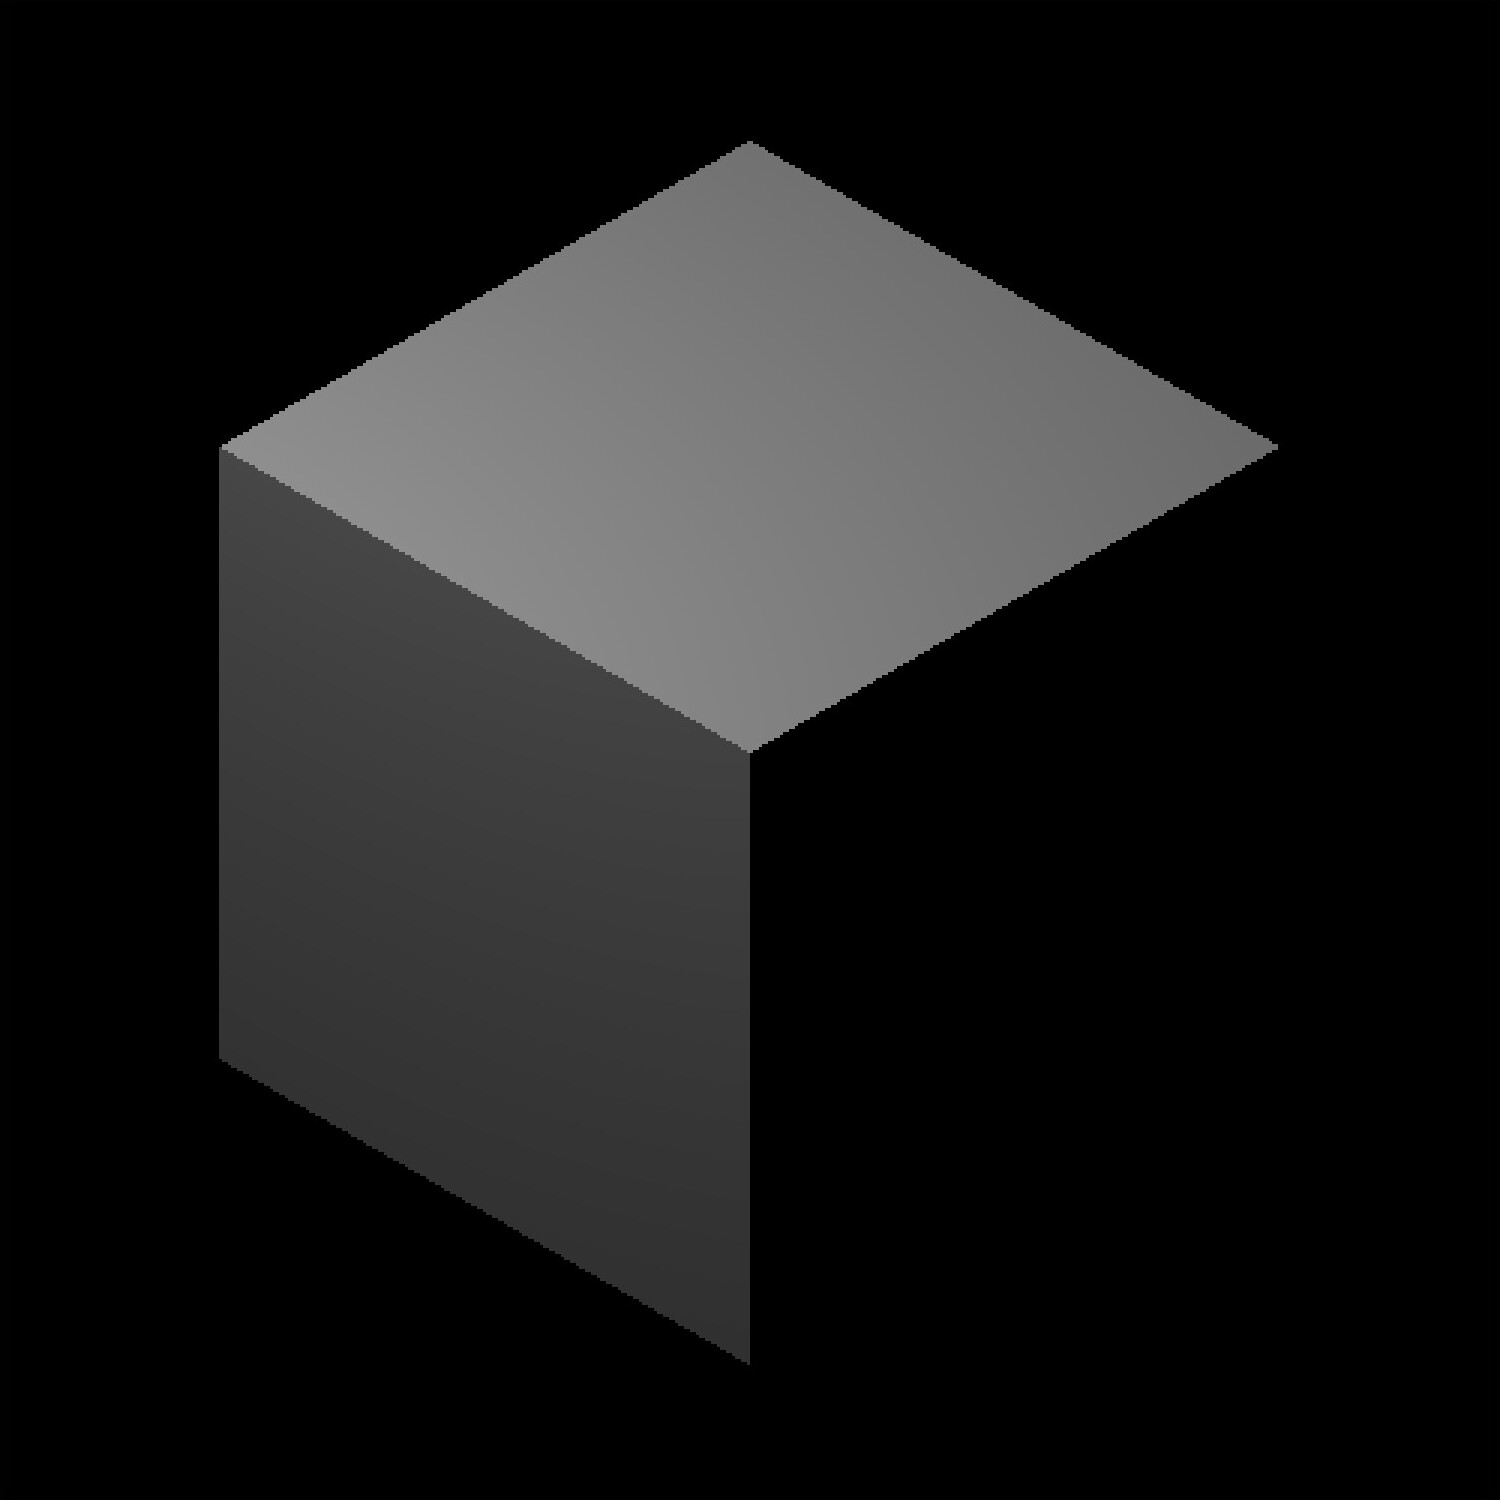
\includegraphics[width=3.8cm]{Cube1.jpg}
%     \end{FigureSub}
%     \hspace{0.5cm}
%     \begin{FigureSub}[Ambient着色]
%         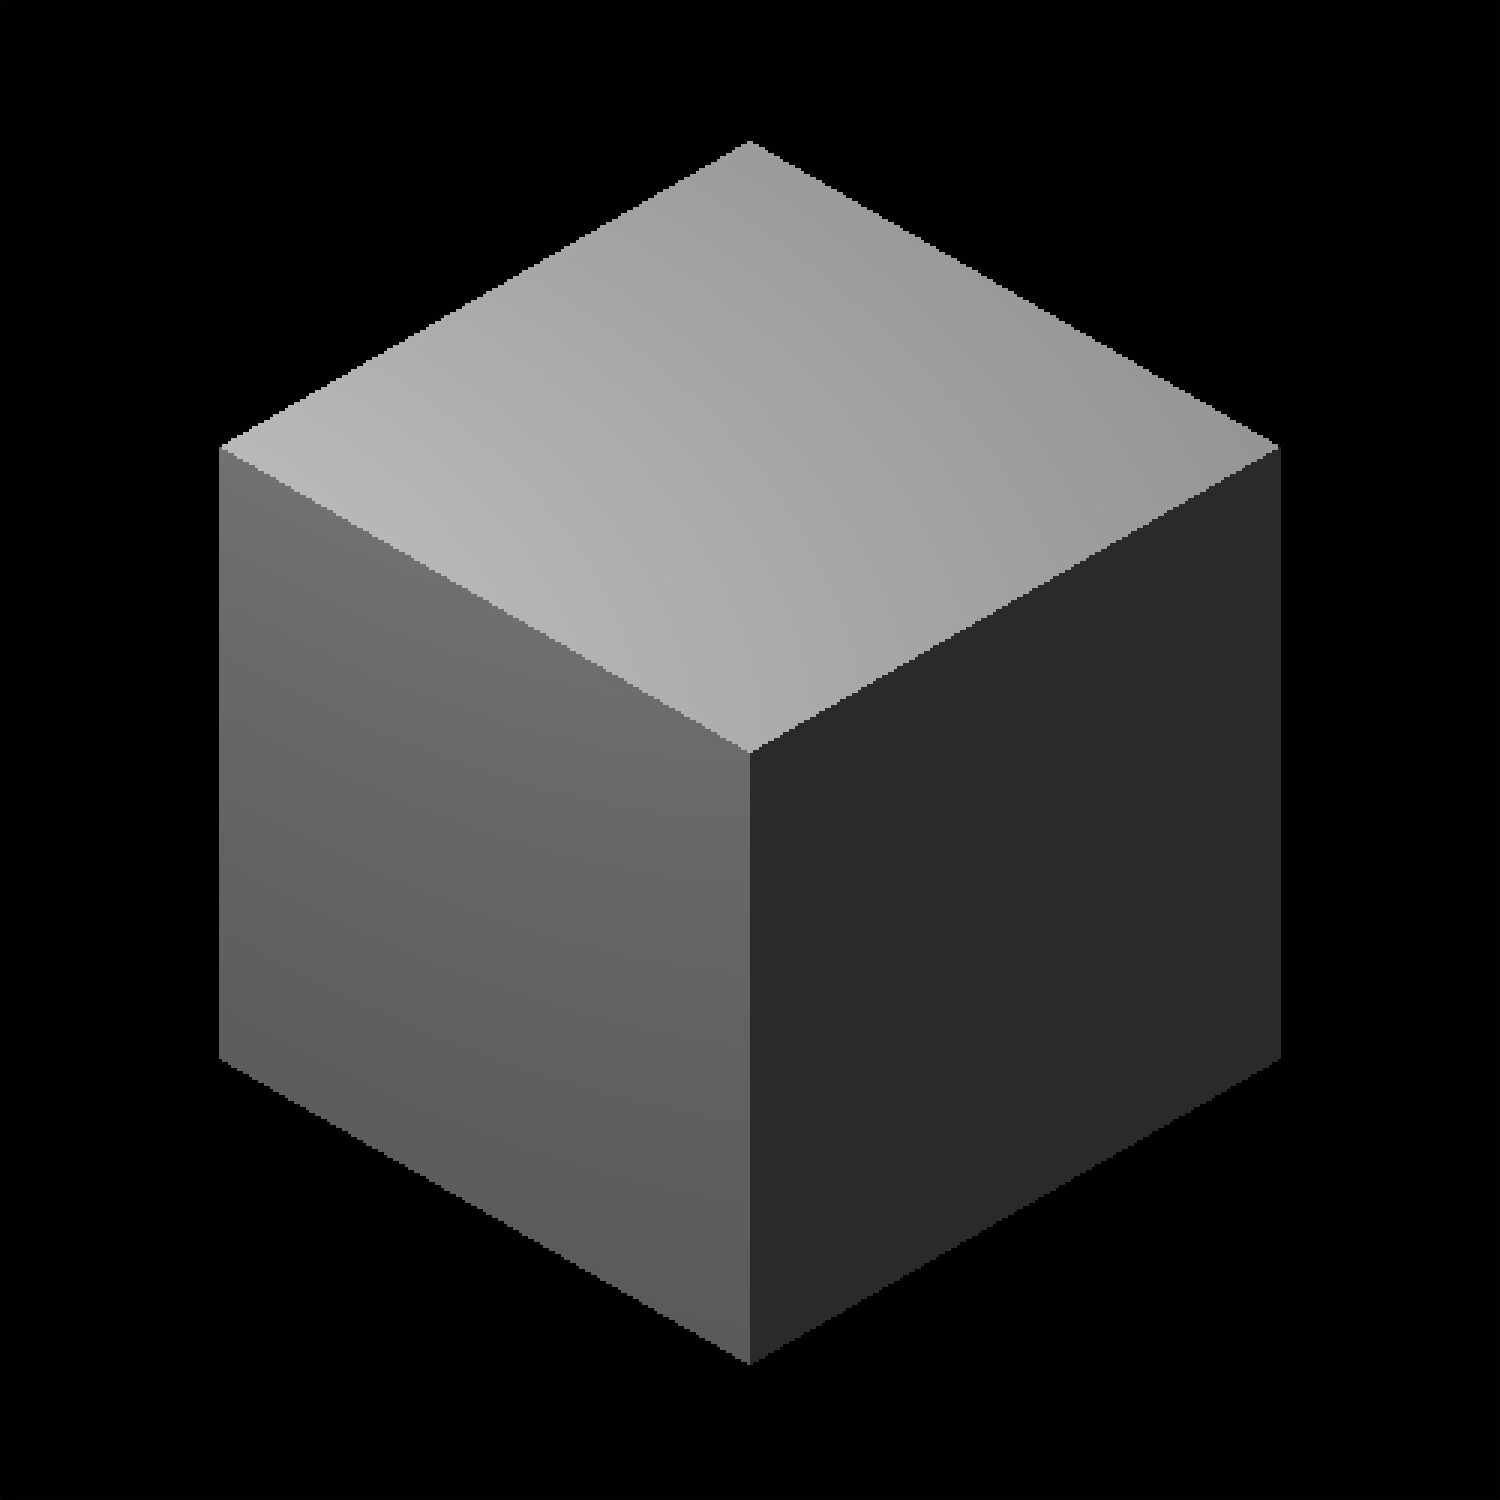
\includegraphics[width=3.8cm]{Cube2.jpg}
%     \end{FigureSub}
% \end{Figure}
% \cref{fig:Lambertian着色}中仅考虑了Lambertian着色,光源从左侧照向立方体。注意到,左侧面和上侧面被不同程度照亮,这是因为光线和左侧面与上侧面的法向量具有不同的夹角,同时,右侧面未被照亮,是全黑的。\cref{fig:Ambient着色}在此基础上添加了Ambient着色,得益于环境光照的引入,右侧面现在不再是完全黑暗的,同时,叠加环境光照后,左侧面和上侧面也比原来更亮了一些。

% \begin{Figure}[Blinn-Phong着色]
%     \begin{FigureSub}[$p=10$;p10]
%         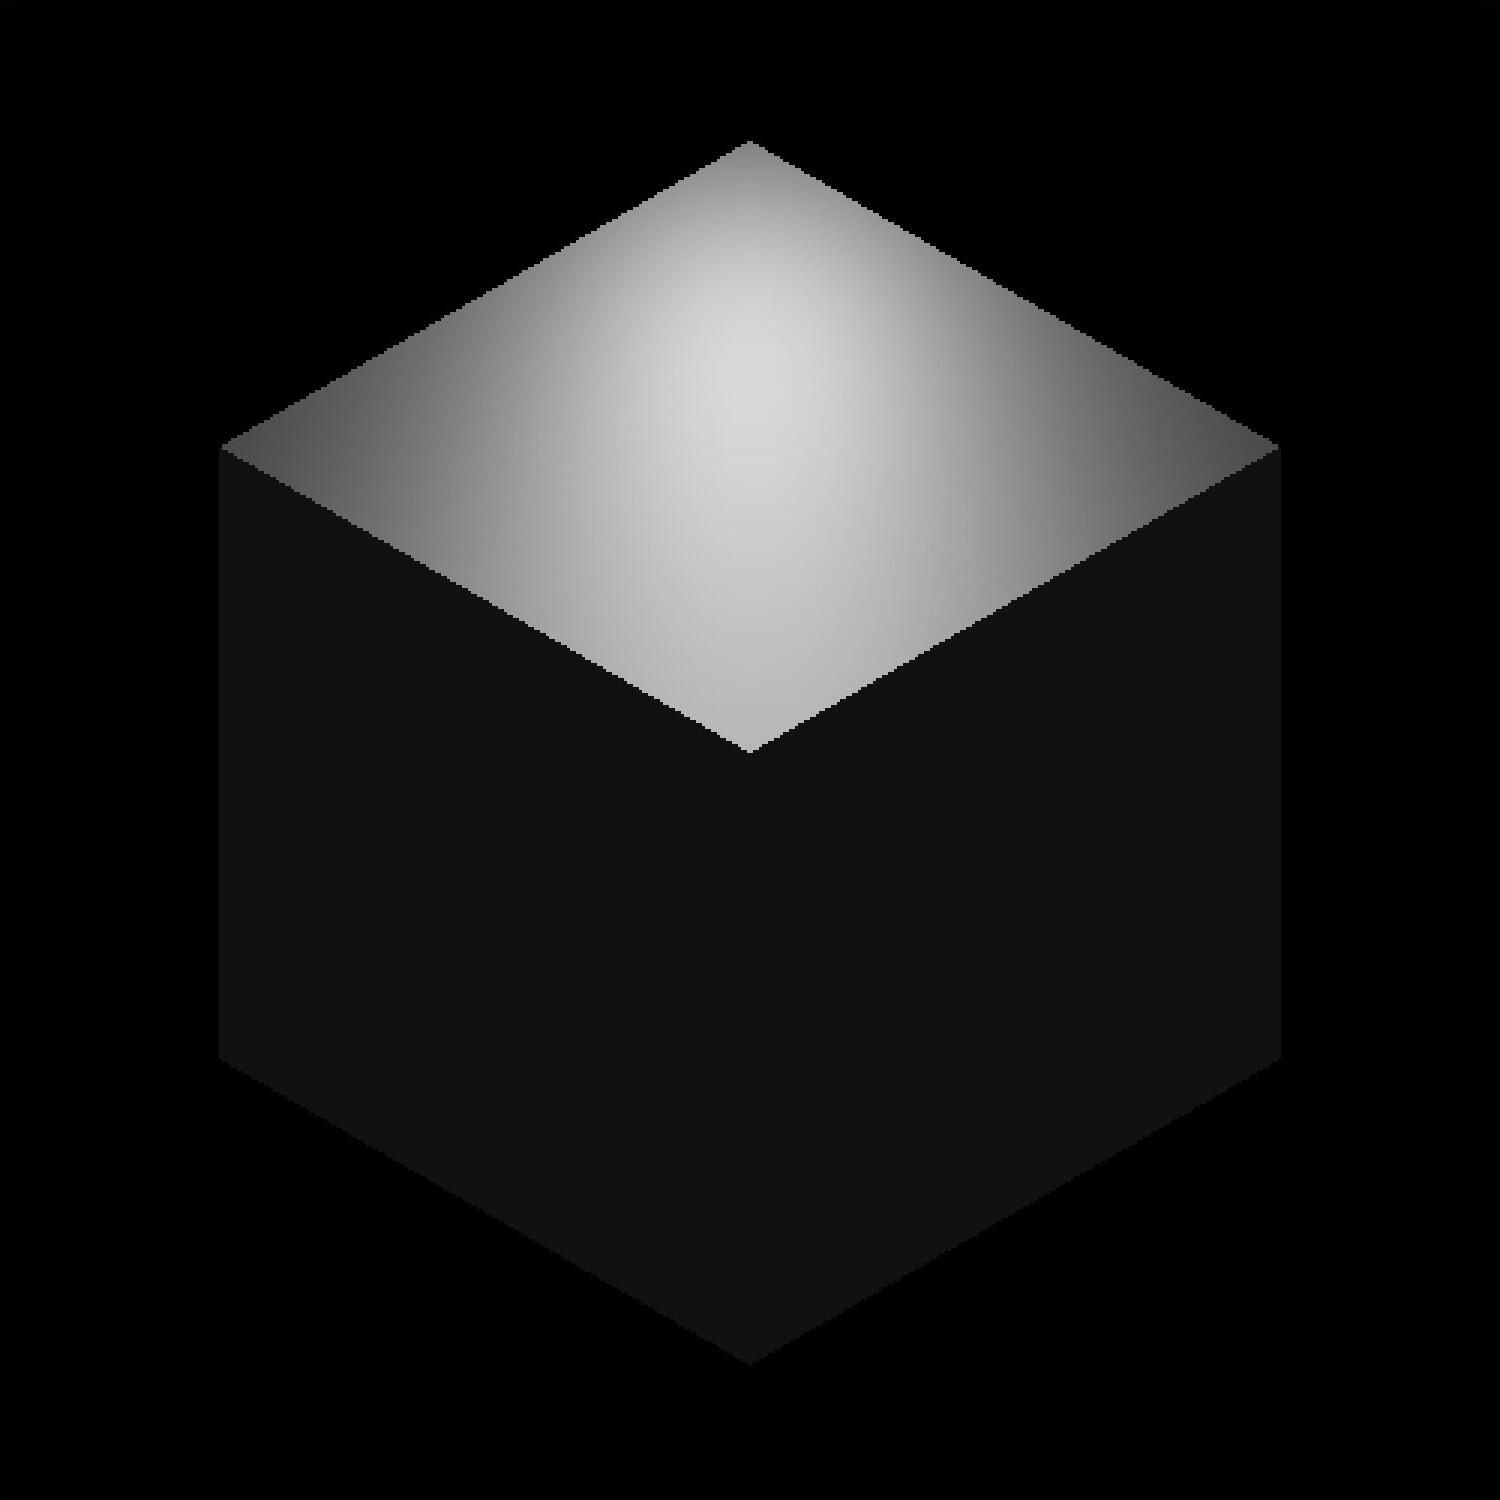
\includegraphics[width=3.8cm]{Cube3.jpg}
%     \end{FigureSub}
%     \hspace{0.5cm}
%     \begin{FigureSub}[$p=100$;p100]
%         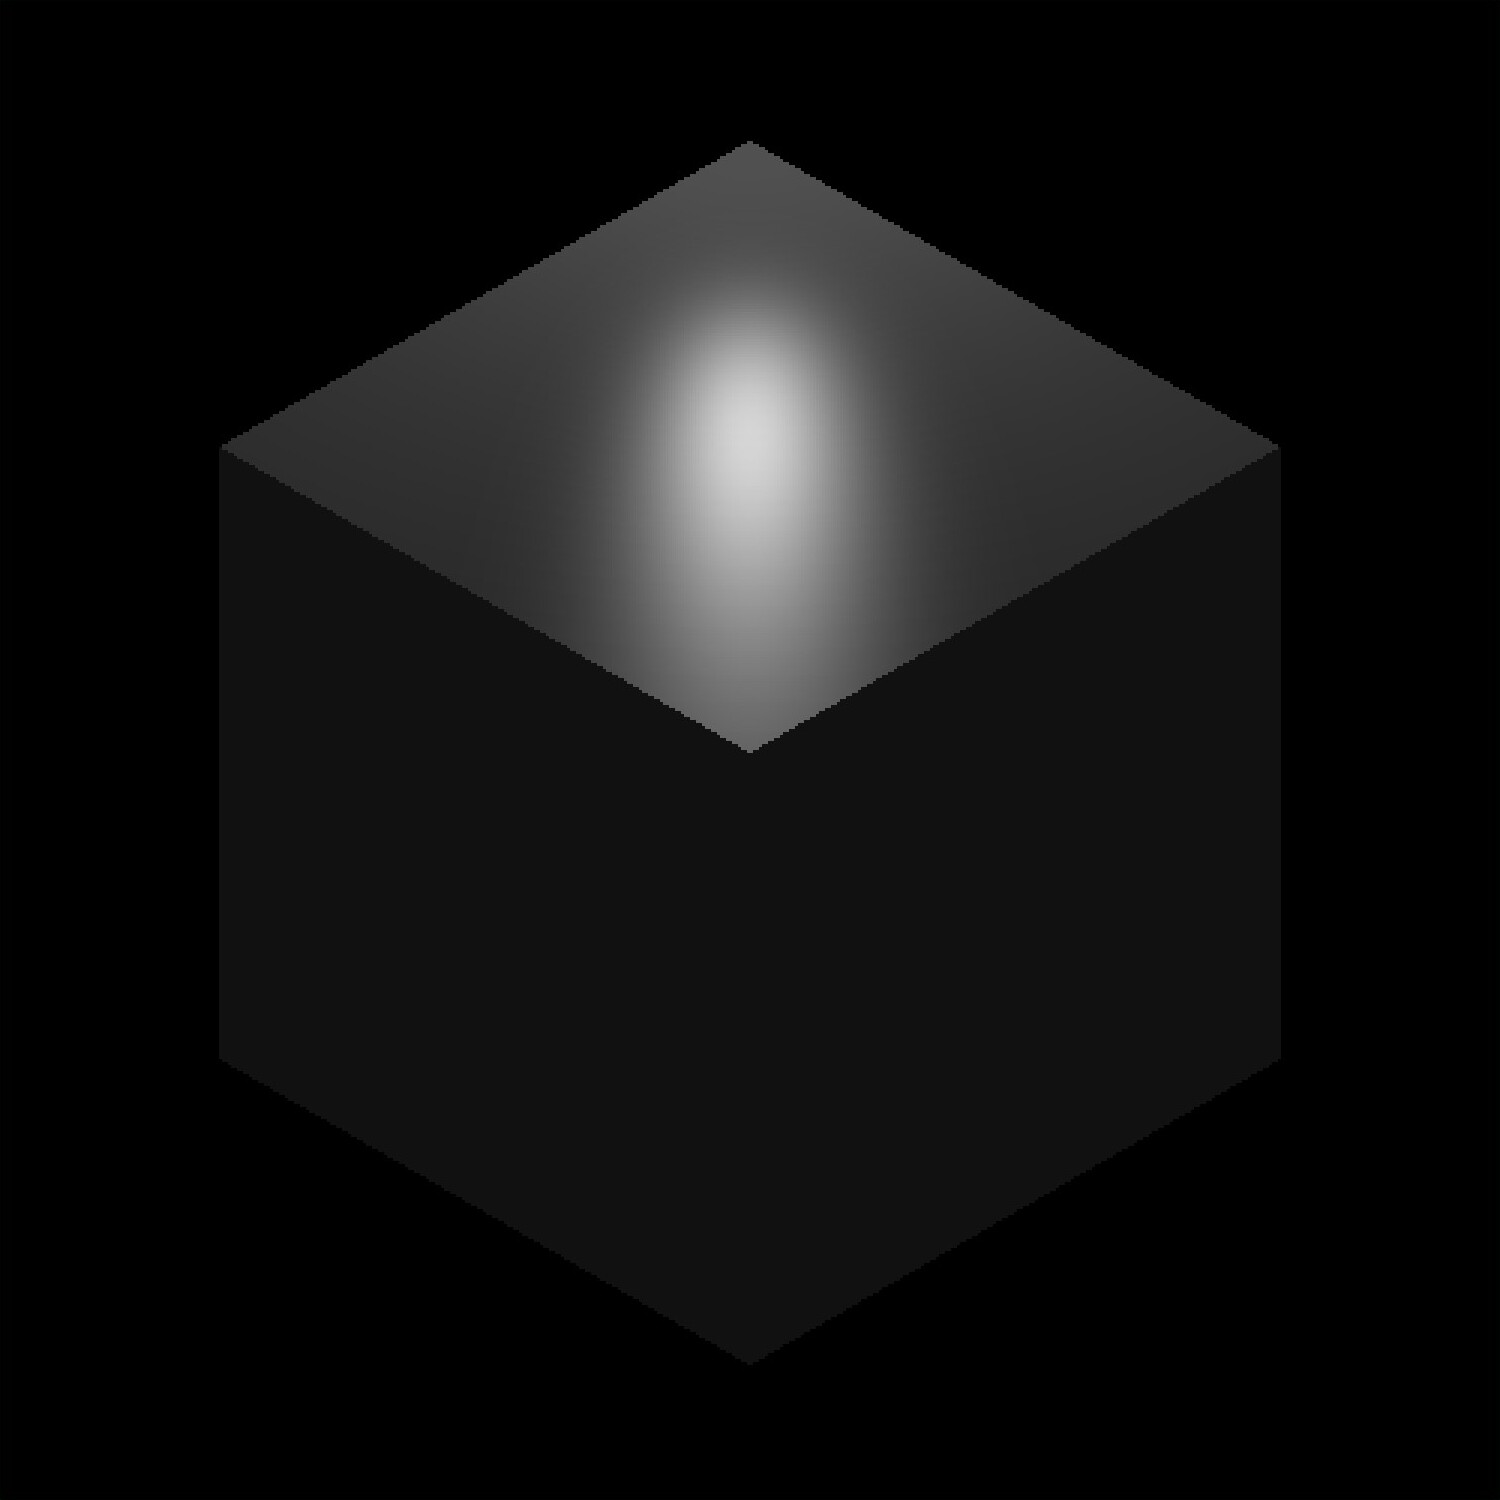
\includegraphics[width=3.8cm]{Cube4.jpg}
%     \end{FigureSub}
%     \hspace{0.5cm}
%     \begin{FigureSub}[$p=1000$;p1000]
%         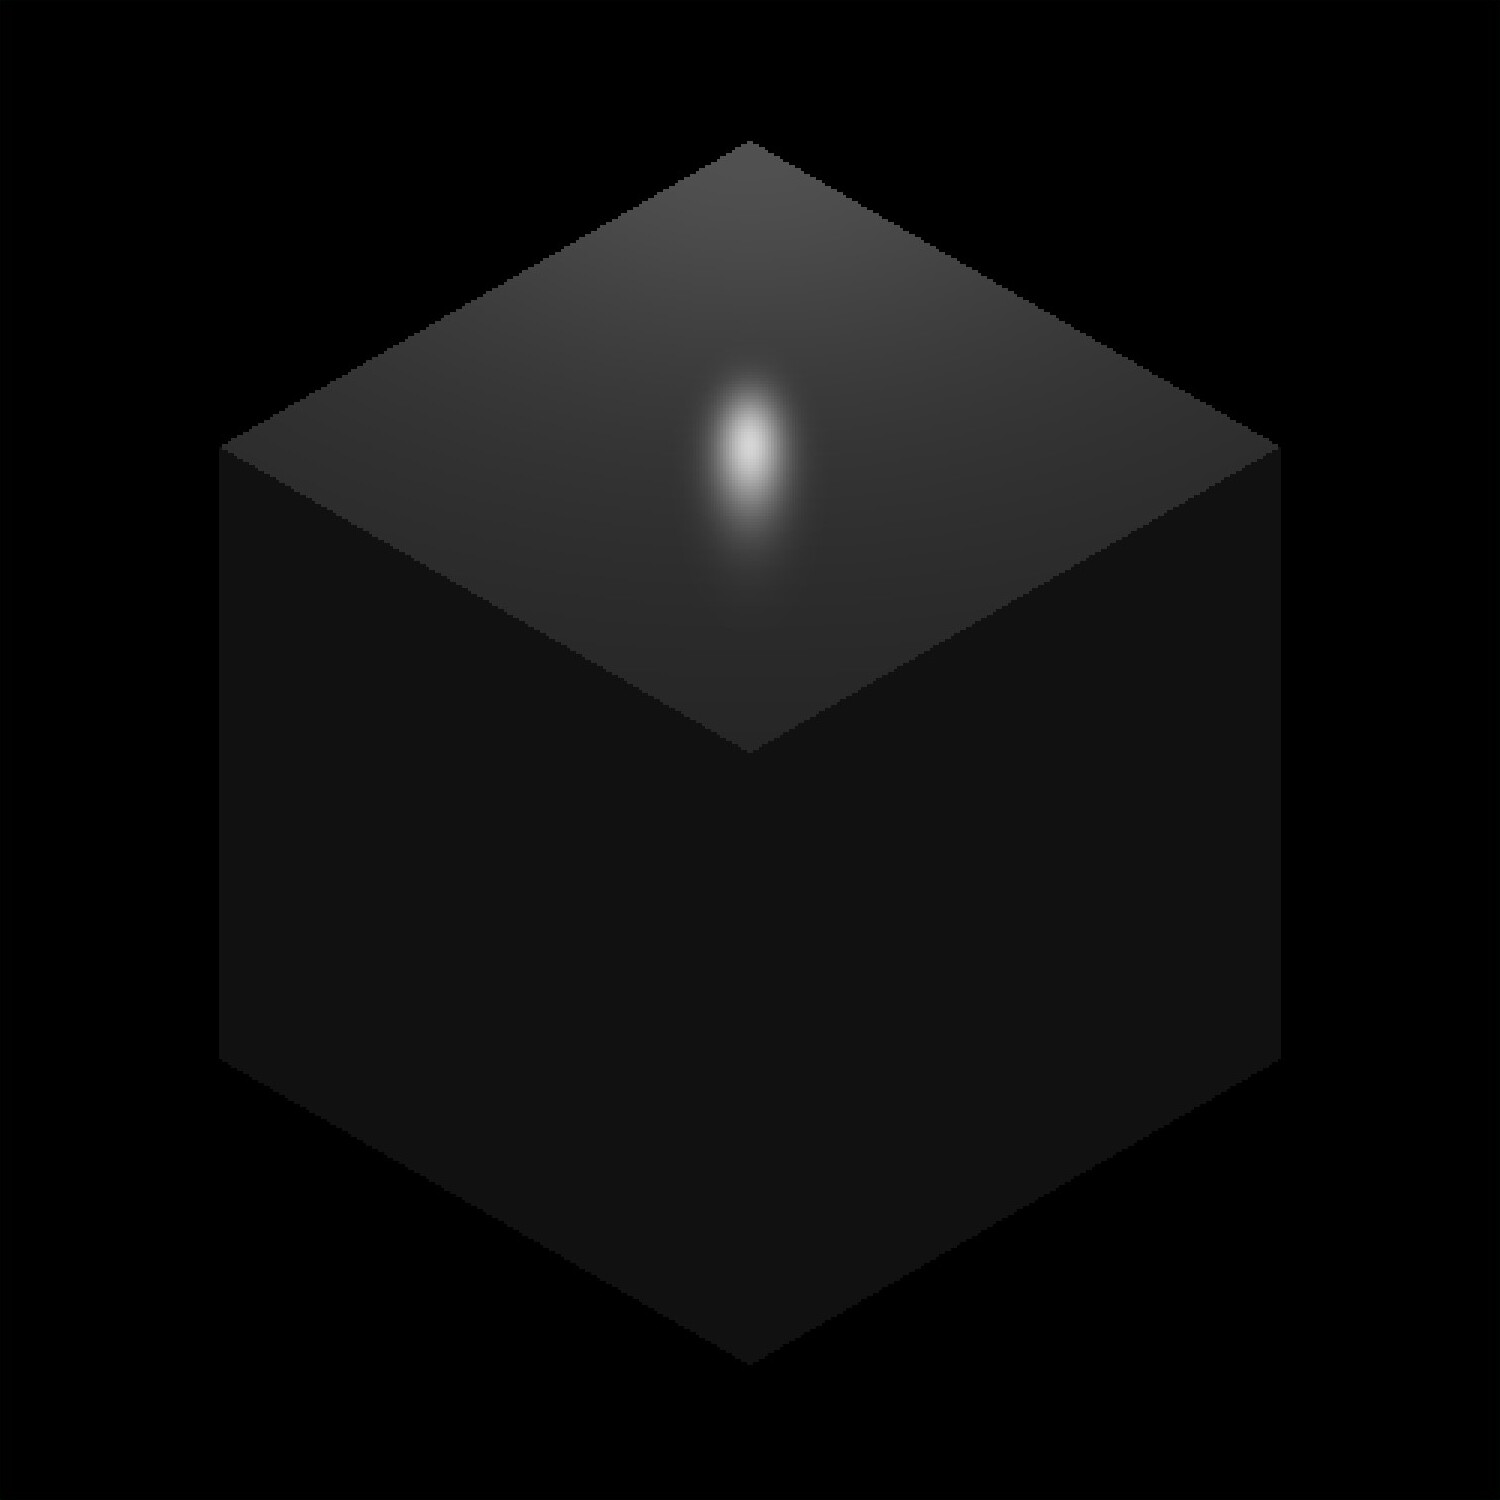
\includegraphics[width=3.8cm]{Cube5.jpg}
%     \end{FigureSub}
% \end{Figure}
% 我们知道,Blinn-Phong着色有效的关键在于,视线需要位于光源反射线上,因此\cref{fig:Lambertian着色和Ambient着色}中的光源布置无法体现Blinn-Phong着色的效果。在\cref{fig:Blinn-Phong着色}中,我们将光源移动至了顶侧,同时降低漫反射颜色$c_d$并增加镜面反射颜色$c_s$以更好凸显高光效果。我们注意到,Blinn-Phong着色使立方体的上侧面表现出了明显的反光,且随着$p$值的增大,高光的光斑就相应越小。
